\section{CBuffer\-Event$<$ T $>$::CGeneric\-Buffer\-Reactor$<$ U $>$  Class Template Reference}
\label{classCBufferEvent_1_1CGenericBufferReactor}\index{CBufferEvent::CGenericBufferReactor@{CBuffer\-Event::CGeneric\-Buffer\-Reactor}}
Inheritance diagram for CBuffer\-Event$<$ T $>$::CGeneric\-Buffer\-Reactor$<$ U $>$::\begin{figure}[H]
\begin{center}
\leavevmode
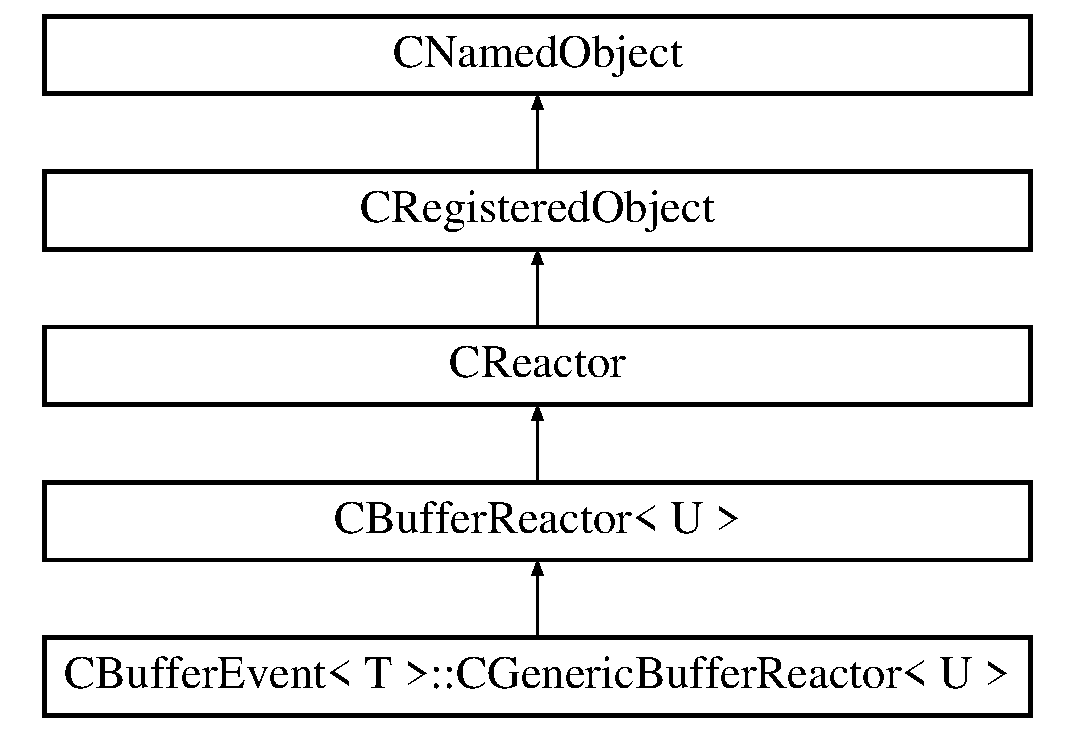
\includegraphics[height=5cm]{classCBufferEvent_1_1CGenericBufferReactor}
\end{center}
\end{figure}
\subsection*{Public Methods}
\begin{CompactItemize}
\item 
{\bf CGeneric\-Buffer\-Reactor} ({\bf CBuffer\-Event}$<$ U $>$ \&owner)
\item 
virtual void {\bf On\-Buffer} ({\bf CBuffer\-Monitor}$<$ T $>$ \&r\-Monitor, Pointer$<$ DAQBuffer$<$ T $>$, T $>$ p\-Buffer)
\item 
virtual void {\bf On\-Timeout} ({\bf CEvent\-Monitor} \&r\-Monitor)
\end{CompactItemize}
\subsection*{Private Attributes}
\begin{CompactItemize}
\item 
{\bf CBuffer\-Event}$<$ U $>$ \& {\bf m\_\-r\-Owner}
\end{CompactItemize}


\subsection{Detailed Description}
\subsubsection*{template$<$class T$>$template$<$class U$>$ class CBuffer\-Event$<$ T $>$::CGeneric\-Buffer\-Reactor$<$ U $>$}

The buffer reactor for {\bf CBuffer\-Event} {\rm (p.\,\pageref{classCBufferEvent})} is actually a nested class: It relays all of the calls back to the event's virtual functions. this allows the presentation of a monolithic model for managing the  events. 



Definition at line 360 of file CBuffer\-Event.h.

\subsection{Constructor \& Destructor Documentation}
\index{CBufferEvent::CGenericBufferReactor@{CBuffer\-Event::CGeneric\-Buffer\-Reactor}!CGenericBufferReactor@{CGenericBufferReactor}}
\index{CGenericBufferReactor@{CGenericBufferReactor}!CBufferEvent::CGenericBufferReactor@{CBuffer\-Event::CGeneric\-Buffer\-Reactor}}
\subsubsection{\setlength{\rightskip}{0pt plus 5cm}template$<$class T$>$ template$<$class U$>$ {\bf CBuffer\-Event}$<$ T $>$::CGeneric\-Buffer\-Reactor$<$ U $>$::CGeneric\-Buffer\-Reactor$<$ U $>$ ({\bf CBuffer\-Event}$<$ U $>$ \& {\em Owner})}\label{classCBufferEvent_1_1CGenericBufferReactor_a0}


Construct a Generic Buffer Reactor. This is the sort of buffer reactor which is associated with a {\bf CBuffer\-Event} {\rm (p.\,\pageref{classCBufferEvent})}. \begin{Desc}
\item[Parameters: ]\par
\begin{description}
\item[{\em 
Owner}]- Owning event. \end{description}
\end{Desc}


\subsection{Member Function Documentation}
\index{CBufferEvent::CGenericBufferReactor@{CBuffer\-Event::CGeneric\-Buffer\-Reactor}!OnBuffer@{OnBuffer}}
\index{OnBuffer@{OnBuffer}!CBufferEvent::CGenericBufferReactor@{CBuffer\-Event::CGeneric\-Buffer\-Reactor}}
\subsubsection{\setlength{\rightskip}{0pt plus 5cm}template$<$class T$>$ template$<$class U$>$ void {\bf CBuffer\-Event}$<$ T $>$::CGeneric\-Buffer\-Reactor$<$ U $>$::On\-Buffer ({\bf CBuffer\-Monitor}$<$ T $>$ \& {\em r\-MOnitor}, Pointer$<$ DAQBuffer$<$ T $>$, T $>$ {\em p\-Buffer})\hspace{0.3cm}{\tt  [virtual]}}\label{classCBufferEvent_1_1CGenericBufferReactor_a1}


Called when a buffer arrives. The Event's On\-Buffer is called with the pointer to the buffer.\begin{Desc}
\item[Parameters: ]\par
\begin{description}
\item[{\em 
r\-Monitor}]- reference to the monitor which fired the event. \item[{\em 
p\-Buffer}]- `Pointer' to the event buffer. \end{description}
\end{Desc}


Definition at line 327 of file CBuffer\-Event.cpp.

References CBuffer\-Event$<$ T $>$::CGeneric\-Buffer\-Reactor$<$ U $>$::m\_\-r\-Owner, and CBuffer\-Event$<$ U $>$::On\-Buffer().\index{CBufferEvent::CGenericBufferReactor@{CBuffer\-Event::CGeneric\-Buffer\-Reactor}!OnTimeout@{OnTimeout}}
\index{OnTimeout@{OnTimeout}!CBufferEvent::CGenericBufferReactor@{CBuffer\-Event::CGeneric\-Buffer\-Reactor}}
\subsubsection{\setlength{\rightskip}{0pt plus 5cm}template$<$class T$>$ template$<$class U$>$ void {\bf CBuffer\-Event}$<$ T $>$::CGeneric\-Buffer\-Reactor$<$ U $>$::On\-Timeout ({\bf CEvent\-Monitor} \& {\em r\-Monitor})\hspace{0.3cm}{\tt  [virtual]}}\label{classCBufferEvent_1_1CGenericBufferReactor_a2}


Called when the buffer monitor times out, but only if the buffer event has been programmed to pass timeouts on to user code. Again, this call is relayed to the Event's On\-Timeout function. \begin{Desc}
\item[Parameters: ]\par
\begin{description}
\item[{\em 
r\-Monitor}]- Reference to the event monitor (unused). \end{description}
\end{Desc}


Reimplemented from {\bf CReactor} {\rm (p.\,\pageref{classCReactor_a8})}.

Definition at line 344 of file CBuffer\-Event.cpp.

References CBuffer\-Event$<$ T $>$::CGeneric\-Buffer\-Reactor$<$ U $>$::m\_\-r\-Owner, and CBuffer\-Event$<$ U $>$::On\-Timeout().

\subsection{Member Data Documentation}
\index{CBufferEvent::CGenericBufferReactor@{CBuffer\-Event::CGeneric\-Buffer\-Reactor}!m_rOwner@{m\_\-rOwner}}
\index{m_rOwner@{m\_\-rOwner}!CBufferEvent::CGenericBufferReactor@{CBuffer\-Event::CGeneric\-Buffer\-Reactor}}
\subsubsection{\setlength{\rightskip}{0pt plus 5cm}template$<$class T$>$ template$<$class U$>$ {\bf CBuffer\-Event}$<$U$>$\& {\bf CBuffer\-Event}$<$ T $>$::CGeneric\-Buffer\-Reactor$<$ U $>$::m\_\-r\-Owner\hspace{0.3cm}{\tt  [private]}}\label{classCBufferEvent_1_1CGenericBufferReactor_o0}




Definition at line 362 of file CBuffer\-Event.h.

Referenced by CBuffer\-Event$<$ T $>$::CGeneric\-Buffer\-Reactor$<$ U $>$::On\-Buffer(), and CBuffer\-Event$<$ T $>$::CGeneric\-Buffer\-Reactor$<$ U $>$::On\-Timeout().

The documentation for this class was generated from the following files:\begin{CompactItemize}
\item 
{\bf CBuffer\-Event.h}\item 
{\bf CBuffer\-Event.cpp}\end{CompactItemize}
